\chapter{Tree Implementation} % Write in your own chapter title
\label{Chapter6}
\lhead{Chapter 6. \emph{Tree Implementation}}

\begin{figure}[H]
	\centering
	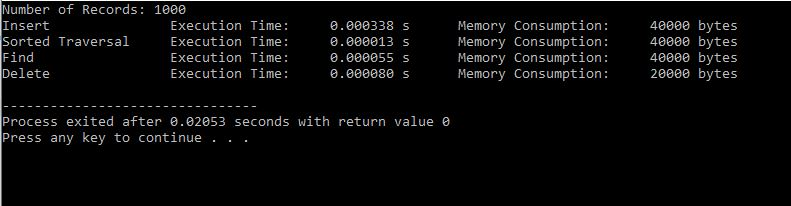
\includegraphics[scale =0.7]{./Figures/Tree1000.jpg}
	\rule{35em}{0.5pt}
	\caption{Results for tree implementation with data size 1000.}
	\label{fig:Tree 1000}
\end{figure}

\begin{figure}[H]
	\centering
	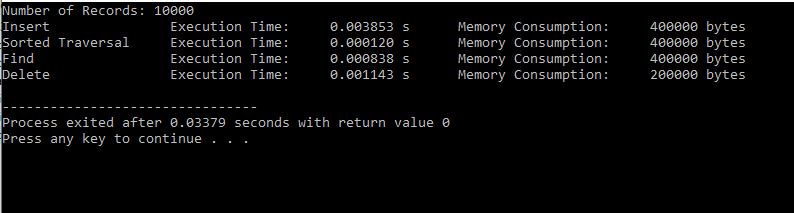
\includegraphics[scale =0.7]{./Figures/Tree10000.jpg}
	\rule{35em}{0.5pt}
	\caption{Results for tree implementation with data size 10000.}
	\label{fig:Tree 10000}
\end{figure}

\begin{figure}[H]
	\centering
	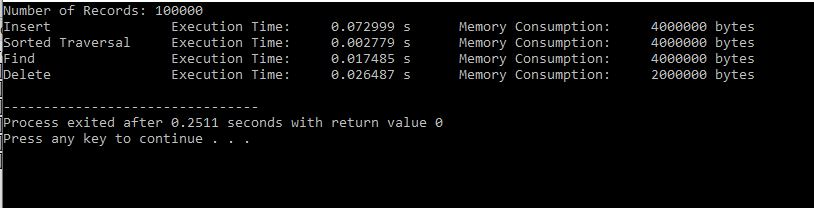
\includegraphics[scale =0.7]{./Figures/Tree100000.jpg}
	\rule{35em}{0.5pt}
	\caption{Results for tree implementation with data size 100000.}
	\label{fig:Tree 100000}
\end{figure}

\begin{figure}[H]
	\centering
	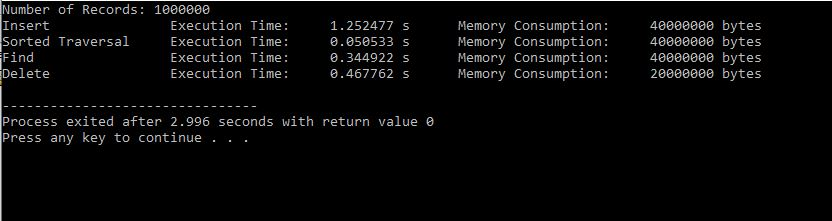
\includegraphics[scale =0.7]{./Figures/Tree1000000.jpg}
	\rule{35em}{0.5pt}
	\caption{Results for tree implementation with data size 1000000.}
	\label{fig:Tree 1000000}
\end{figure}
